\resizebox{\textwidth}{!}{
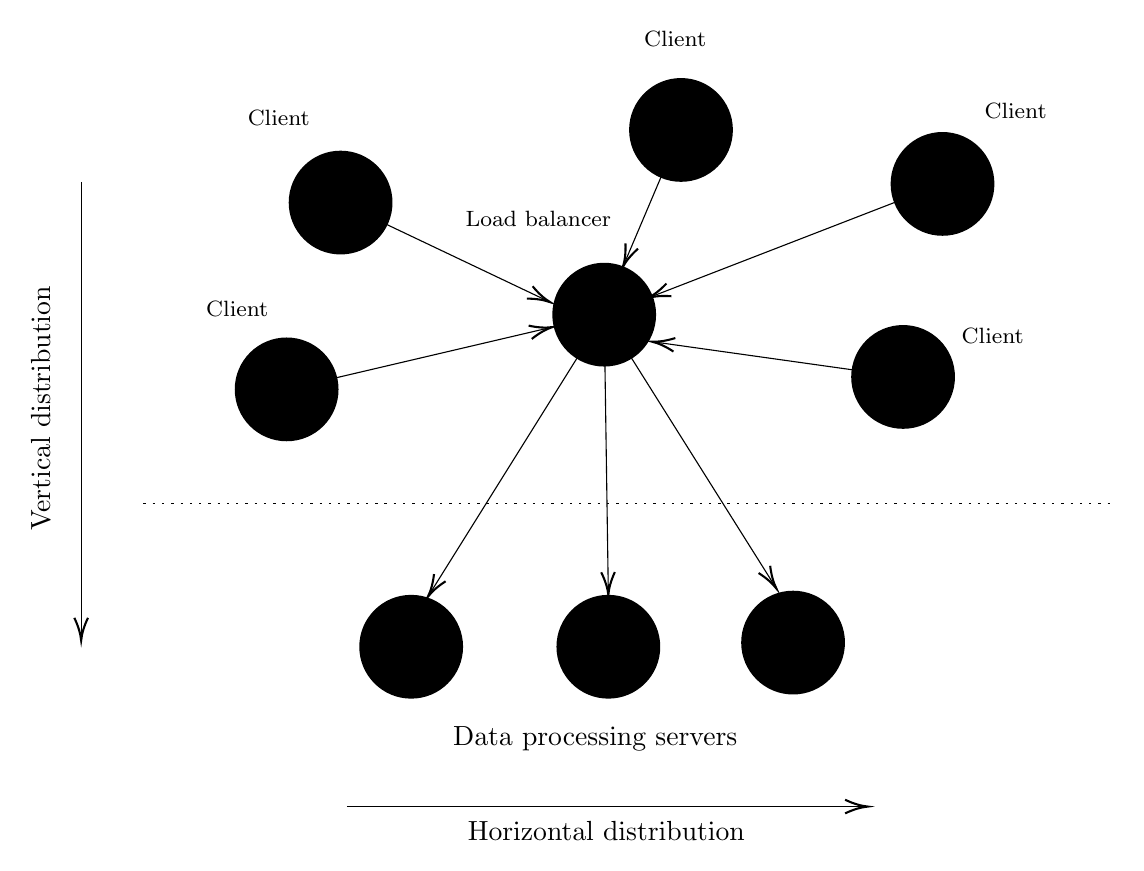
\begin{tikzpicture}[x=0.75pt,y=0.75pt,yscale=-1,xscale=1]
%uncomment if require: \path (0,451); %set diagram left start at 0, and has height of 451

%Shape: Circle [id:dp21625012916250363] 
\draw  [draw opacity=0][fill={rgb, 255:red, 0; green, 0; blue, 0 }  ,fill opacity=1 ] (307,172) .. controls (307,158.19) and (318.19,147) .. (332,147) .. controls (345.81,147) and (357,158.19) .. (357,172) .. controls (357,185.81) and (345.81,197) .. (332,197) .. controls (318.19,197) and (307,185.81) .. (307,172) -- cycle ;
%Shape: Circle [id:dp4205702906990445] 
\draw  [draw opacity=0][fill={rgb, 255:red, 0; green, 0; blue, 0 }  ,fill opacity=1 ] (451,202) .. controls (451,188.19) and (462.19,177) .. (476,177) .. controls (489.81,177) and (501,188.19) .. (501,202) .. controls (501,215.81) and (489.81,227) .. (476,227) .. controls (462.19,227) and (451,215.81) .. (451,202) -- cycle ;
%Shape: Circle [id:dp1834367315754477] 
\draw  [draw opacity=0][fill={rgb, 255:red, 0; green, 0; blue, 0 }  ,fill opacity=1 ] (470,109) .. controls (470,95.19) and (481.19,84) .. (495,84) .. controls (508.81,84) and (520,95.19) .. (520,109) .. controls (520,122.81) and (508.81,134) .. (495,134) .. controls (481.19,134) and (470,122.81) .. (470,109) -- cycle ;
%Shape: Circle [id:dp8062304220658076] 
\draw  [draw opacity=0][fill={rgb, 255:red, 0; green, 0; blue, 0 }  ,fill opacity=1 ] (344,83) .. controls (344,69.19) and (355.19,58) .. (369,58) .. controls (382.81,58) and (394,69.19) .. (394,83) .. controls (394,96.81) and (382.81,108) .. (369,108) .. controls (355.19,108) and (344,96.81) .. (344,83) -- cycle ;
%Shape: Circle [id:dp3524619405588886] 
\draw  [draw opacity=0][fill={rgb, 255:red, 0; green, 0; blue, 0 }  ,fill opacity=1 ] (214,332) .. controls (214,318.19) and (225.19,307) .. (239,307) .. controls (252.81,307) and (264,318.19) .. (264,332) .. controls (264,345.81) and (252.81,357) .. (239,357) .. controls (225.19,357) and (214,345.81) .. (214,332) -- cycle ;
%Shape: Circle [id:dp2671841919001372] 
\draw  [draw opacity=0][fill={rgb, 255:red, 0; green, 0; blue, 0 }  ,fill opacity=1 ] (309,332) .. controls (309,318.19) and (320.19,307) .. (334,307) .. controls (347.81,307) and (359,318.19) .. (359,332) .. controls (359,345.81) and (347.81,357) .. (334,357) .. controls (320.19,357) and (309,345.81) .. (309,332) -- cycle ;
%Shape: Circle [id:dp3753155355544049] 
\draw  [draw opacity=0][fill={rgb, 255:red, 0; green, 0; blue, 0 }  ,fill opacity=1 ] (398,330) .. controls (398,316.19) and (409.19,305) .. (423,305) .. controls (436.81,305) and (448,316.19) .. (448,330) .. controls (448,343.81) and (436.81,355) .. (423,355) .. controls (409.19,355) and (398,343.81) .. (398,330) -- cycle ;
%Shape: Circle [id:dp9331094894799612] 
\draw  [draw opacity=0][fill={rgb, 255:red, 0; green, 0; blue, 0 }  ,fill opacity=1 ] (180,118) .. controls (180,104.19) and (191.19,93) .. (205,93) .. controls (218.81,93) and (230,104.19) .. (230,118) .. controls (230,131.81) and (218.81,143) .. (205,143) .. controls (191.19,143) and (180,131.81) .. (180,118) -- cycle ;
%Shape: Circle [id:dp15130202099269585] 
\draw  [draw opacity=0][fill={rgb, 255:red, 0; green, 0; blue, 0 }  ,fill opacity=1 ] (154,208) .. controls (154,194.19) and (165.19,183) .. (179,183) .. controls (192.81,183) and (204,194.19) .. (204,208) .. controls (204,221.81) and (192.81,233) .. (179,233) .. controls (165.19,233) and (154,221.81) .. (154,208) -- cycle ;
%Straight Lines [id:da6549389594791377] 
\draw    (205,118) -- (304.19,165.14) ;
\draw [shift={(306,166)}, rotate = 205.42] [color={rgb, 255:red, 0; green, 0; blue, 0 }  ][line width=0.75]    (10.93,-3.29) .. controls (6.95,-1.4) and (3.31,-0.3) .. (0,0) .. controls (3.31,0.3) and (6.95,1.4) .. (10.93,3.29)   ;
%Straight Lines [id:da41842174722404835] 
\draw    (179,208) -- (305.05,178.46) ;
\draw [shift={(307,178)}, rotate = 166.81] [color={rgb, 255:red, 0; green, 0; blue, 0 }  ][line width=0.75]    (10.93,-3.29) .. controls (6.95,-1.4) and (3.31,-0.3) .. (0,0) .. controls (3.31,0.3) and (6.95,1.4) .. (10.93,3.29)   ;
%Straight Lines [id:da5248390031839211] 
\draw    (369,83) -- (341.78,147.16) ;
\draw [shift={(341,149)}, rotate = 292.99] [color={rgb, 255:red, 0; green, 0; blue, 0 }  ][line width=0.75]    (10.93,-3.29) .. controls (6.95,-1.4) and (3.31,-0.3) .. (0,0) .. controls (3.31,0.3) and (6.95,1.4) .. (10.93,3.29)   ;
%Straight Lines [id:da3704088342799581] 
\draw    (495,109) -- (354.86,163.28) ;
\draw [shift={(353,164)}, rotate = 338.83] [color={rgb, 255:red, 0; green, 0; blue, 0 }  ][line width=0.75]    (10.93,-3.29) .. controls (6.95,-1.4) and (3.31,-0.3) .. (0,0) .. controls (3.31,0.3) and (6.95,1.4) .. (10.93,3.29)   ;
%Straight Lines [id:da45067791114233546] 
\draw    (476,202) -- (356.98,185.28) ;
\draw [shift={(355,185)}, rotate = 8] [color={rgb, 255:red, 0; green, 0; blue, 0 }  ][line width=0.75]    (10.93,-3.29) .. controls (6.95,-1.4) and (3.31,-0.3) .. (0,0) .. controls (3.31,0.3) and (6.95,1.4) .. (10.93,3.29)   ;
%Straight Lines [id:da675702571699395] 
\draw    (332,172) -- (248.06,306.3) ;
\draw [shift={(247,308)}, rotate = 302.01] [color={rgb, 255:red, 0; green, 0; blue, 0 }  ][line width=0.75]    (10.93,-3.29) .. controls (6.95,-1.4) and (3.31,-0.3) .. (0,0) .. controls (3.31,0.3) and (6.95,1.4) .. (10.93,3.29)   ;
%Straight Lines [id:da19941562676333713] 
\draw    (332,172) -- (333.97,305) ;
\draw [shift={(334,307)}, rotate = 269.15] [color={rgb, 255:red, 0; green, 0; blue, 0 }  ][line width=0.75]    (10.93,-3.29) .. controls (6.95,-1.4) and (3.31,-0.3) .. (0,0) .. controls (3.31,0.3) and (6.95,1.4) .. (10.93,3.29)   ;
%Straight Lines [id:da44186877727070717] 
\draw    (332,172) -- (413.94,302.31) ;
\draw [shift={(415,304)}, rotate = 237.84] [color={rgb, 255:red, 0; green, 0; blue, 0 }  ][line width=0.75]    (10.93,-3.29) .. controls (6.95,-1.4) and (3.31,-0.3) .. (0,0) .. controls (3.31,0.3) and (6.95,1.4) .. (10.93,3.29)   ;
%Straight Lines [id:da00352783652063271] 
\draw  [dash pattern={on 0.84pt off 2.51pt}]  (110,263) -- (578,263) ;
%Straight Lines [id:da8513516782413686] 
\draw    (80,108) -- (80,327) ;
\draw [shift={(80,329)}, rotate = 270] [color={rgb, 255:red, 0; green, 0; blue, 0 }  ][line width=0.75]    (10.93,-3.29) .. controls (6.95,-1.4) and (3.31,-0.3) .. (0,0) .. controls (3.31,0.3) and (6.95,1.4) .. (10.93,3.29)   ;
%Straight Lines [id:da5994970572513846] 
\draw    (208,409) -- (457,409) ;
\draw [shift={(459,409)}, rotate = 180] [color={rgb, 255:red, 0; green, 0; blue, 0 }  ][line width=0.75]    (10.93,-3.29) .. controls (6.95,-1.4) and (3.31,-0.3) .. (0,0) .. controls (3.31,0.3) and (6.95,1.4) .. (10.93,3.29)   ;

% Text Node
\draw (264,121) node [anchor=north west][inner sep=0.75pt]   [align=left] {{\footnotesize Load balancer}};
% Text Node
\draw (159,72) node [anchor=north west][inner sep=0.75pt]   [align=left] {{\footnotesize Client}};
% Text Node
\draw (350,34) node [anchor=north west][inner sep=0.75pt]   [align=left] {{\footnotesize Client}};
% Text Node
\draw (514,69) node [anchor=north west][inner sep=0.75pt]   [align=left] {{\footnotesize Client}};
% Text Node
\draw (503,177) node [anchor=north west][inner sep=0.75pt]   [align=left] {{\footnotesize Client}};
% Text Node
\draw (139,164) node [anchor=north west][inner sep=0.75pt]   [align=left] {{\footnotesize Client}};
% Text Node
\draw (258,369) node [anchor=north west][inner sep=0.75pt]   [align=left] {Data processing servers};
% Text Node
\draw (54.5,277.5) node [anchor=north west][inner sep=0.75pt]  [rotate=-270] [align=left] {Vertical distribution};
% Text Node
\draw (265,415) node [anchor=north west][inner sep=0.75pt]   [align=left] {Horizontal distribution};


\end{tikzpicture}
}
